% Setup - do not change
\documentclass[11pt]{article}
\usepackage[top=0.9in, left=0.9in, bottom=0.9in, right=0.9in]{geometry} 
\usepackage{parskip}

\usepackage[english]{babel}
\usepackage[utf8]{inputenc}
\usepackage{amsmath,amsthm,amssymb,graphicx,pdfpages,lipsum,hyperref}
\usepackage[none]{hyphenat}
\usepackage{csquotes}

\setlength\parindent{0pt}
%%%%%%%%%%%%%%%%%%%%%%%%%%%%%%%%%%%%%%%%%%%%%%%%%%%%%%%%%%%%%%%%%%%
% add other packages here if required
\usepackage{subcaption}
\usepackage{wrapfig}
\usepackage{amsfonts}
\usepackage{booktabs}
\usepackage{siunitx}
\usepackage{mwe}


%% Bibliography are specified in this file. You can also choose inline bib style if you want to. But make sure your citation style is consistent (and proper)
% For more details on citation: https://library.unimelb.edu.au/recite
\usepackage[sorting = none]{biblatex}
\addbibresource{references.bib}
\usepackage{url}
\setcounter{biburllcpenalty}{7000}
\setcounter{biburlucpenalty}{8000}

%%%%%%%%%%%%%%%%%%%%%%%%%%%%%%%%%%%%%%%%%%%%%%%%%%%%%%%%%%%%%%%%%%% the '%' symbol denotes comments

% Begin document creation
\title{\textbf{Predicting Hourly Zone Profitability for Yellow Taxis in NYC}}
\author{
James La Fontaine \\
Student ID: 1079860 \\
%% Replace the link with your github repo
% 1. Remember to escape underscore (\_) in the link.
% 2. Remember to include the commit you want to submit in the link
\href{INSERT GITHUB REPO HERE i.e https://github.com/MAST30034-Applied-Data-Science/mast30034-project-1-jameslafontaine}{Github repo with commit}
}

\begin{document}
\maketitle

\section{Introduction}
% Link to a 30 min tutorial if you require revision: https://www.overleaf.com/learn/latex/Learn_LaTeX_in_30_minutes

Traditional taxi companies have been slow to incorporate new technologies to optimise dispatching and routing, and thus remain inefficient.  They typically employ a roomful of human dispatchers, each communicating using outdated radio technology. Dispatchers are often required to be former drivers who rely on their lifetime of road experience, with some not even taking advantage of digital maps \cite{routingInefficiency}. This has undoubtedly been one of the several key factors involved in allowing ridesharing companies such as Uber and Lyft to surpass traditional taxis in the private transport service industry \cite{taxiVsUber}. To make matters worse, traditional taxi drivers face long work hours and high costs including their fuel costs and the cost of owning or leasing a taxi medallion, which reached prices as high as \$1 million in the early 2010s in New York City (NYC) \cite{taxiVsUber}.

It is the aim of this report to investigate which factors determine the hourly profitability of a taxi zone in NYC based on the taxi zones defined by the NYC Taxi \& Limousine Commission (TLC) \cite{taxizones}. Two different Machine Learning models will be presented which utilise the various factors that will be investigated in an attempt to predict hourly taxi zone profitability. The findings of this investigation and models produced will be of interest to both taxi drivers and taxi companies located within the NYC region (and potentially across different regions depending on which factors are found to be most important). With the provided information, said drivers and companies should be able to markedly improve their routing and dispatch systems, maximising both efficiency and profitability.

\subsection{Datasets}
\textbf{TLC Yellow Taxi Trip Record Data} sourced from the NYC TLC \cite{taxidata} will be the main dataset used for this investigation. The trip records consist of information about each trip (such as pickup and dropoff time and location, fare amount, etc.) completed in NYC yellow taxis within a given month. Only yellow taxi trips will be considered as they make up a large majority of taxi trips in New York City and can respond to street-hails in any taxi zone. The time period looked at will be May-November 2022, as this period is post-COVID and occurred just before changes were made to NYC taxi fare pricing in December 2022. This time period should still be recent enough to provide relevant data for the purposes of this investigation. This dataset contains \textbf{23,585,385 taxi trips} between May and November 2022 before filtering.

\newpage

The following assumptions will be made about the yellow taxi trip record business rules \cite{taxidatadict} and dataset:

\begin{itemize} 
    \item The overnight and rush hour extra surcharges are applied based on pickup time, and only one of these surcharges can apply for a given trip. 
    \item The maximum amount of passengers can never exceed 6 based on Driver Rule 54-15(g) in Chapter 54 of the TLC rule book. \cite{passengerlaw}
    \item The minimum fare amount during the time period of these taxi trips was \$2.50 for yellow taxis. \cite{oldfare}
    \item The NYS congestion surcharge during the time period of these taxi trips was \$2.50, based on how often this value appears in the data
    \item The \$0.50 MTA tax doesn't apply to trips that end in Newark, based on the data and TLC taxi fare page. \cite{taxifarepage}
    \item A trip is recorded within the year and month in which pickup occurred.
    \item Trips shorter than 1 minute or a quarter mile \cite{walkingdistance} are to be considered erroneous as it is reasonable to expect people to only use taxis for trips longer than this.
\end{itemize} 

In addition to this taxi data, external datasets were gathered to assist in the analysis and prediction of hourly taxi zone profitability. These datasets include:
\begin{itemize} 
    \item \textbf{MTA NYCT Subway Entrances and Exits: 2015} - Contains the entrances and exits at New York City Subway stations, which includes but is not limited to: Division, Line, Station Name, and Longitude and Latitude coordinates. The dataset was grouped by subway station before being downloaded on data.ny.gov and after doing so contains \textbf{472 records} of each train station location in NYC. \cite{externalsubway}
    \item \textbf{Insideairbnb New York City Airbnb Listing Data (04 December, 2022)} - Summary information and metrics for Airbnb listings in NYC updated as of December 4th, 2022. \textbf{41533 records} each containing various information about Airbnb listings such as price, location (latitude and longitude), minimum nights available, etc. \cite{externalairbnb}
    \item \textbf{Hotels Properties Citywide} - Contains information about hotels within the five NYC boroughs, including their latitude and longitude. \textbf{5519 records}. \cite{externalhotels}
    \item \textbf{New York City Census Data 2015 5-Year Estimates} - Contains a selection of NYC census data (total population, racial/ethnic demographic information, employment and commuting characteristics, etc.). The data is split up into the different NYC census tracts. The longitude and latitude of the blocks in which census data is aggregated are also provided in a separate file to allow geospatial analysis after the blocks have been merged into the appropriate tracts they're contained in \footnote{Note that tracts are geographic regions defined for the purpose of taking a census and blocks are a further subdivision of tracts}. $\approx$ \textbf{2100 records.} \cite{externalcensus}
    \item \textbf{Parking Meters Locations and Status} - Contains recent data (2023) such as status and longitude, latitude of multiple space parking Muni-Meters located along streets and within municipal parking facilities where metered parking is available \footnote{Muni Meter is the name used by the New York City Department of Transportation (NYCDOT) for its pay and display centralized parking meter system}. \textbf{13415 records}. \cite{externalparking}
\end{itemize} 

It is assumed for the older and newer datasets that the data will still be relevant enough to allow for a legitimate analysis due to the steady nature of train station counts, parking meters, census statistics (in terms of how locations rank amongst each other), etc. This has the added benefit of not requiring models utilising such information to possess constantly up-to-date data to perform well.

% Example here used biblatex to manage citations: https://www.overleaf.com/learn/latex/Bibliography_management_with_biblatex , You are free to choose your own way for managing references if biblatex seems too hard.

% You can have \section{}, \subsection{}, and \subsubsection{}, \section*{}, \subsection*{}, and \subsubsection*{}
\section{Preprocessing}
\subsection{Filtering and Cleaning using Business Logic}
The following records were removed from the yellow taxi trip data using business logic contained in the data dictionary \cite{taxidatadict} and the assumptions stated in the Introduction:

\begin{itemize} 
    \item \textbf{Records with negative or invalid fares / other fees}. For example, fare amount being less than \$2.50, overnight or rush hour surcharges being applied outside of the timeslots specified in the data dictionary, incorrect congestion surcharge amount applied, airport fee being applied to a non-airport pickup or not being applied to a JFK or LaGuardia  airport pickup, etc.
    \item \textbf{Records that did not occur within the relevant range of pickup and dropoff locations}. This investigation only looks at taxi zones numbered between 1-263 as this covers all of NYC.
    \item \textbf{Records with invalid passenger amounts}. There should be at least 1 passenger for each valid trip but less than or equal to 6 based on the passenger count assumption stated earlier.
    \item \textbf{Trips that did not occur with the standard, JFK or Newark rates}. This investigation is solely concerned with standard trips within NYC and the airports so other rates aren't relevant.
    \item \textbf{Records containing invalid Vendor IDs}. Only Vendor IDs of 1 and 2 are considered valid according to the data dictionary.
    \item \textbf{Negative or less than 1/4 mile or 1 minute trip distance records}. Based on the assumption stated earlier.
    \item \textbf{Records where the payment type was not a credit card}. As tips are only automatically recorded for credit card payment, proper analysis involving tips can only be performed if trips involving other payment types are removed.
    \item \textbf{Records where the total amount does not equal the sum of the other fees}. If the other fees did not add up to the total amount, then the record was simply treated as erroneous.
    \item \textbf{Records where the trip did not begin in the month of the dataset}. In accordance with the assumption stated earlier, if a trip does not begin in the same month as the dataset that its contained in, then it is assumed to be erroneous.
    \item \textbf{Records containing NULL values}. Records containing NULL values were assumed to be erroneous, and analysis and modelling will be a lot easier without these records due to imputation not being simplistic for this data due to the dependence between features. This would also provide flexibility in the event that pyspark.ml were to be used, which does not handle NULL values well.
\end{itemize} 

The yellow taxi trip data ended up containing \textbf{9,355,380 records} after filtering / cleaning.

The following filtering and cleaning was performed on the external datasets:

\begin{itemize} 
    \item Hotels recorded under the 2022 financial year were extracted to provide the most relevant hotel information.
    \item Only parking Muni-Meters recorded as 'Active' were retained.
\end{itemize} 

\subsection{Feature Engineering and Aggregation}
For the yellow taxi data, boolean features denoting whether a trip occurred on a weekday and / or public holiday were included, with public holidays for NYC in 2022 being referenced from OfficeHolidays \cite{holidays}. Month, day of week, day of month, and hour were extracted from the datetime features. Tolls were subtracted from each trips total, and trip times in minutes were calculated for each trip and used to calculate average USD\$ / minute and average  USD\$ / $\frac{1}{5}$ mile as these are the units used for fare calculations. Average USD\$ / $\frac{1}{5}$ mile and per minute were grouped by location and hour, and number of hourly pickups performed within each location were recorded. A 'zone profitability' metric was created which was equal to the sum of average USD\$ / minute and average USD\$ / $\frac{1}{5}$ mile multiplied by the number of trips within a pickup location for that hour. This metric was intended to combine the taxi demand within a location with the money generated by trips in that zone such that taxi zones with similar demand could be ranked on how efficiently they generate cash. Since most of the yellow taxi trip features had already been used for data filtering, they were removed and only the date, time and pickup location features were retained alongside the newly engineered features which captured all the fee-related information that would be required.

External data feature engineering involved: 
\begin{itemize} 
    \item \textbf{MTA NYCT Subway Entrances and Exits: 2015} - Converting latitude and longitude into a point and merging with the taxi zone geometry data from the TLC website \cite{taxidata}. Then the number of train stations located within each taxi zone was counted and other features were removed. \textbf{153 records}.
    \item \textbf{Insideairbnb New York City Airbnb Listing Data (04 December, 2022)} - Converting latitude and longitude into a point and merging with the taxi zone geometry data from the TLC website. Then the number of airbnbs located within each taxi zone was counted and the average daily airbnb price of each taxi zone was recorded. Other features were removed. \textbf{244 records}.
    \item \textbf{Hotels Properties Citywide} - Converting latitude and longitude into a point and merging with the taxi zone geometry data from the TLC website. Then the number of hotels located within each taxi zone was counted and other features were removed. \textbf{171 records}.
    \item \textbf{New York City Census Data 2015 5-Year Estimates} -  Extracting census tract codes from each census block code in the census\_block\_loc. The latitude and longitudes of each block were averaged to approximate a middle point for each census tract and these were merged with the taxi zone geometry data from the TLC websites. Then wealth, employment, and commuting related features were retained and grouped by each taxi zone, with other features being removed. \textbf{252 records.} 
    \item \textbf{Parking Meters Locations and Status} - Converting latitude and longitude into a point and merging with the taxi zone geometry data from the TLC website. Then the number of parking Muni-Meters located within each taxi zone was counted and other features were removed. \textbf{222 records}.
\end{itemize} 

All data was aggregated by pickup location ID and the combined dataset has a total of \textbf{332,627 records} containing the above information for any given hour on any given day (between May and November 2022) for each individual taxi zone.

\section{Analysis and Visualisation}

Note that the full dataset was used for visualisation due to its smaller size after being grouped into hourly records.

\subsection{Imputation}

Null values for the external features were investigated and addressed. It was decided that null values for census features would be imputed via the median as the median would likely be closer to the true value for regions that are missing data due to the positive skewness of the census data. Null values for other features (number of hotels, number of parking Muni-Meters, number of subway stations in a location, etc.) were assumed to be zero or close to zero based on the fact that these are counts and it would be unlikely for the data to be missing these values / records if these regions had a significant amount of these things. Therefore, null values for these features were imputed with zero. Note that these features are inappropriate for the airport zones and so will not be considered for any analysis or modelling involving the airports.

\subsection{Geospatial and Temporal Analysis}

Due to the positive skewness of hourly trip demand by location (and by extension hourly zone profitability), the log of zone profitability was used during geospatial visualisation to facilitate comparison between all the taxi zones.
From (Figure \ref{1a}), we can see that LaGuardia and JFK Airports (marked by the two blue markers on the right side of the map) are hotspots in terms of taxi profitability. This high demand could likely be explained by the fact that there are huge amounts of people travelling to and from airports who prefer, or even require, the use of taxis.  We can also see in (Figure \ref{1a}) that a large portion of taxi activity occurs in the CBD / Midtown Manhattan (circled in black in the middle). It would be reasonable to assume that this is due to the large amount of people who live and work in this area of NYC. 

A clear relationship between the hour of the day and taxi zone profitability is visible in (Figure \ref{1b}), where we can see that zone profitability picks up after roughly 5am when people start waking up for work on a weekday, and has another surge during rush hour between 4-8pm when people are starting to come home from work. We can also see that zone profitability tends to be lower throughout the whole day on days where people aren't working such as the weekend or public holidays. This further supports the idea that a large portion of taxi customers are people commuting to work, indicating that zone profitability is strongly tied to the amount of people who need to travel to work in a particular area.

\begin{figure}[h]
\centering
\begin{subfigure}{.5\textwidth}
  \centering
  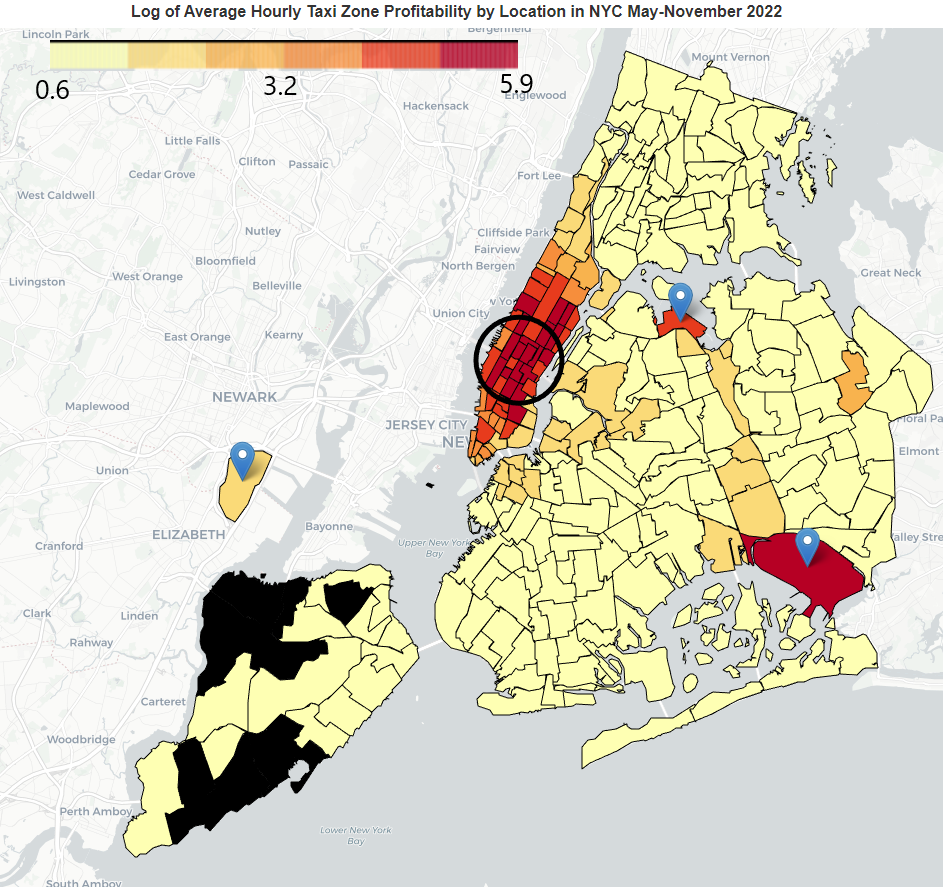
\includegraphics[width=.95\linewidth]{plots/log_zone_prof_map_edit.png}
  \caption{Geospatial Distribution}
  \label{1a}
\end{subfigure}%
\begin{subfigure}{.5\textwidth}
  \centering
  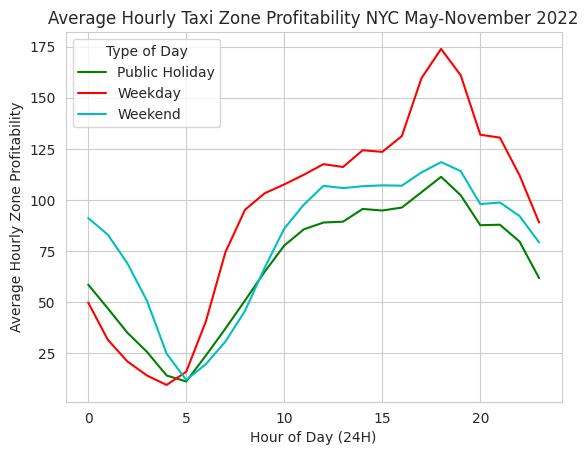
\includegraphics[width=1\linewidth]{plots/temporal_zone_profitability.png}
  \caption{Temporal Distribution}
  \label{1b}
\end{subfigure}
\setlength{\belowcaptionskip}{-10pt}
\caption{Geospatial and Temporal Distribution of NYC Hourly Zone Profitability}
\label{1}
\end{figure}


\subsection{External Data Analysis}
From (Figure \ref{2}) we can see that zone profitability correlates with many of the features extracted from the external datasets. For example, being closer (i.e. shorter commute time) to the CBD / locations where the majority of the `professional' jobs \footnote{Professional jobs are defined as business, management and science jobs in the census data used} are located positively correlates with higher average income per capita and zone profitability. This could also explain why the percentage of people who claim to prefer walking is higher in these zones compared to other areas of NYC, as their workplace is likely within reasonable walking distance for many of them.  The number of parking munimeters being higher within these zones would make sense considering the sheer amount of people working within these zones during the day. 

It is also assumed that the average daily airbnb price being higher within these zones can be explained by the increased wealth and demand of living / staying in these areas, enabling hosts to charge greater prices for their Airbnbs. Additionally, the percentage of people claiming to be self employed or working at home being higher within these areas is likely explained by a greater concentration of business owners being present within these areas. These business owners would identify themselves as self-employed and also be more likely to have the flexibility to work at home. It seems reasonable to conclude that the wealthier and more densely populated an area is, and the higher the amount of private business and management jobs located within it, the more likely taxis are to maximise profit within such areas.

\begin{wrapfigure}{r}{0.5\textwidth}
    \centering
    \vspace{-70pt}
    % change the scale multiplier to make the figures smaller or larger
    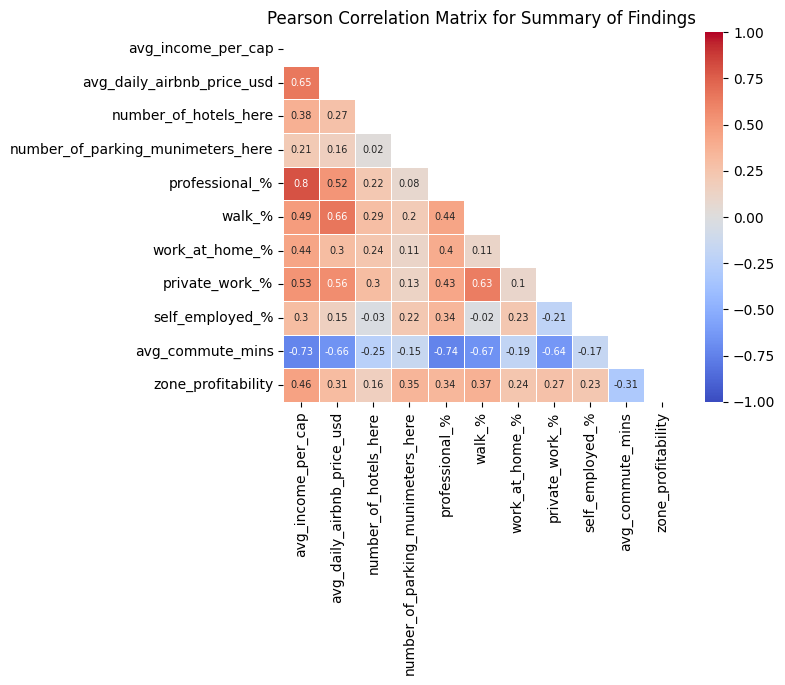
\includegraphics[width=0.6\textwidth]{plots/correlation.png}
    % this ensures your figures are centered where possible

    \caption{External Data Correlation Matrix}
    \vskip -35pt 
    \label{2}
\end{wrapfigure}

\section{Modelling}
Four separate Linear Regression and eXtreme Gradient Boosting Regression models ended up being fitted (two for airport zones, two for the rest of NYC) as the external dataset features were not applicable to airport zones. The response variable of these models was hourly taxi zone profitability. It was assumed that all the features specified below and utilised in all models are available to taxi companies and drivers at the beginning of any given hour and are sufficiently up-to-date. This means that the models produced can be used for future zone profitability predictions. The models were trained on the first 6 months of data (May 2022 to October 2022) and were tested on the November 2022 data.

\subsection{Linear Regression}
Linear regression is a simple and highly interpretable regression model that can be utilised in the case where there exists both categorical and numerical predictors for a numerical response variable \cite{LsmLtfrm}. It was assumed that there is no interaction present between these features. All suitable features in the dataset (hour, day, location, external data features for non-airport zones, etc.) were used after one-hot encoding was applied to categorical features.  



\subsection{eXtreme Gradient Boosting Regression}
In an attempt to improve upon the performance of a linear regression model, an eXtreme Gradient Boosting regression model was utilised. eXtreme Gradient Boosting, or XGBoost for short, is an efficient open-source implementation of the gradient boosting algorithm. Gradient boosting algorithms are ensemble machine learning algorithms that can be used for classification or regression problems. Ensembles are constructed from decision tree models in which trees are added one at a time to the ensemble and fit to correct the prediction errors made by prior models. This is a type of ensemble machine learning model referred to as boosting. Models are fit using any arbitrary differentiable loss function and gradient descent optimization algorithm \cite{XGB}. Hyperopt was used to fine tune the hyperparameters for the XGBoost Regression models and resulted in some performance gain. Hyperopt is a python library which utilises Bayesion optimisation to tune parameters \cite{hyperopt}. Similarly to the linear regression models, all suitable features were used after categorical features were one-hot encoded. 
\section{Results \& Discussion}



\begin{wraptable}{r}{0.35\textwidth}
\vspace{-20pt}
\begin{tabular}{lcc} \toprule
    {\textbf{Model}} & {\textbf{RMSE}} & {$R^2$} \\ \midrule
    LRAirports  & 65.14 & 0.534       \\
    XGBAirports  & \textbf{45.11} & \textbf{0.777}  \\ \midrule
    LRCity  & 84.46  & 0.617       \\
    XGBCity  & \textbf{45.62} & \textbf{0.888}    \\ \bottomrule
    
\end{tabular}
\caption{Model performance on \\ test set}
\label{t1}
\end{wraptable}

From (Table \ref{t1}), we can see that the XGBoost regression model outperformed the linear regression model in both goodness-of-fit ($R^2$) and predictive error (RMSE). (Figure \ref{3}) also supports this with the XGBoost model's predictions (Figure \ref{3c}) closely matching the geospatial distribution of the actual average hourly taxi zone profitability for November 2022(Figure \ref{3a}). Conversley, the linear regression model tended to overestimate all of the less profitable zones as seen in (Figure \ref{3b}). This is likely due to the fact that linear regression is unable to capture the more complex non-linear relationships which may be present between the features and zone profitability. 

As the Root Mean Square Error (RMSE) is in the same units as the response variable, we can say that an average error of roughly 45 for zone profitability is an acceptable level of error when considering that the average hourly zone profitability for hotspots sits above 200, and reaches 400 for the most profitable zones. Furthermore, the XGBoost model appears to retain the relative rankings of important zones fairly well and thus would be suitable for choosing where to go based on the ranking of a zone's profitability. The only reason to select the linear regression model over the XGBoost model would be if interpretability were the main concern. However, taxi companies and taxi drivers will likely care more about model performance than interpretability, especially if the model were to be used for automatic routing.

\begin{figure}[h]
\centering
\begin{subfigure}{.36\textwidth}
    \centering
    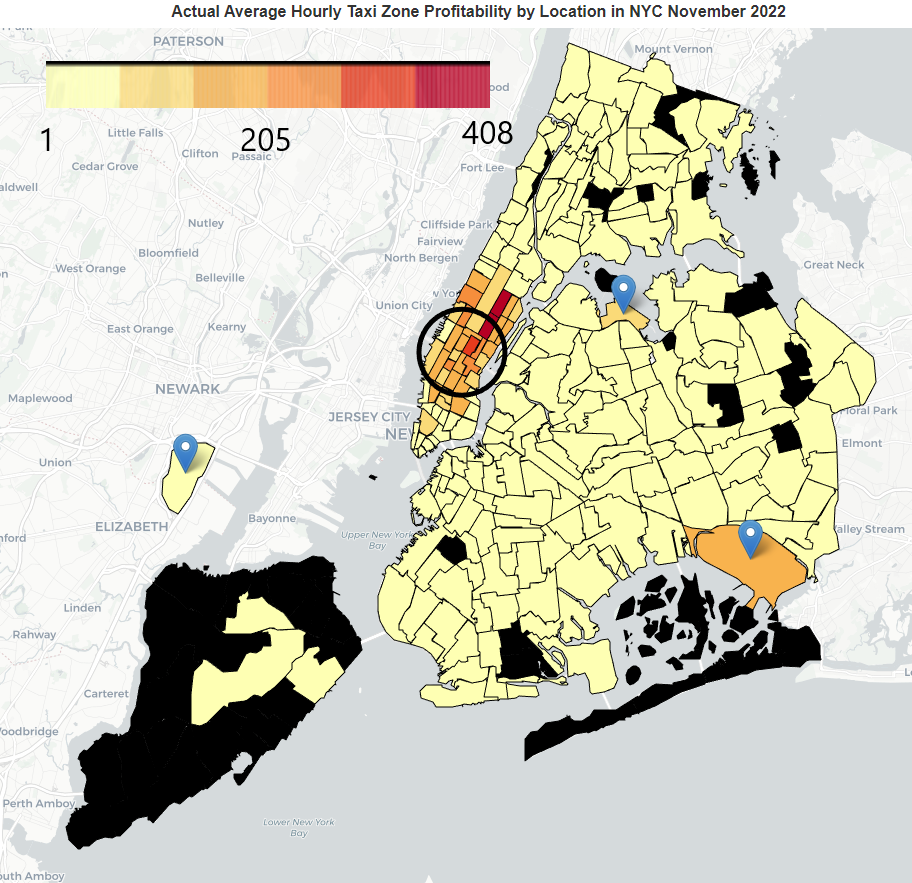
\includegraphics[width=1\linewidth]{plots/modelling_actual_map_edit.png}  
    \caption{Actual}
    \label{3a}
\end{subfigure}
\begin{subfigure}{.36\textwidth}
    \centering
    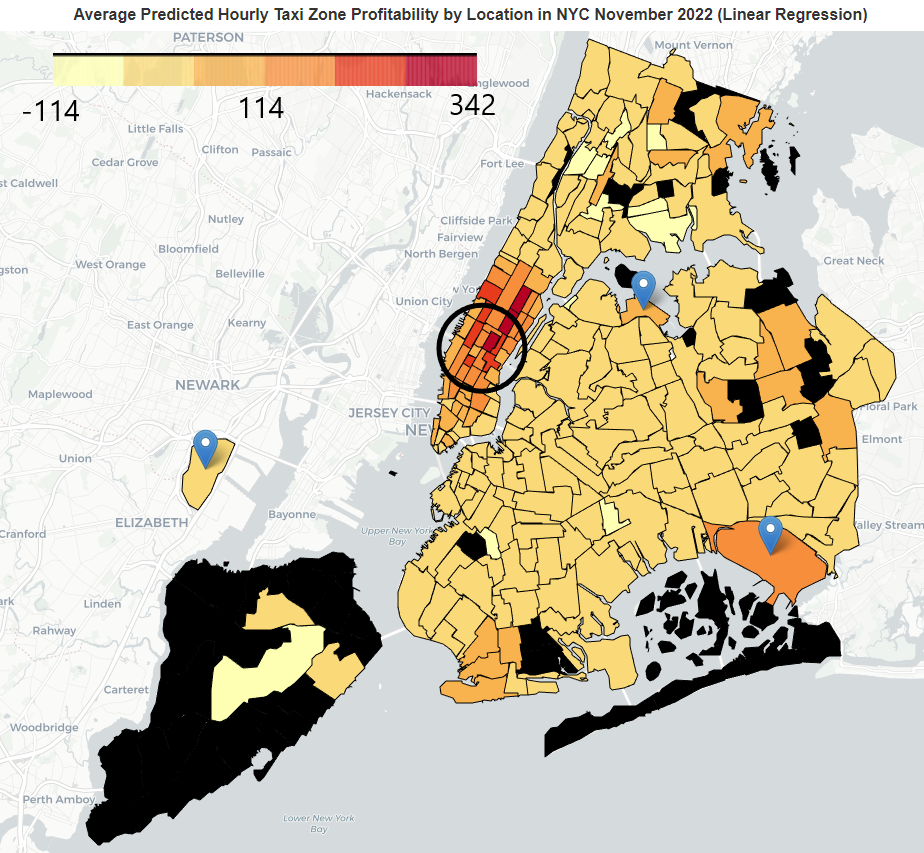
\includegraphics[width=1\linewidth]{plots/modelling_map_LR_edit.png}  
    \caption{Linear Regression}
    \label{3b}
\end{subfigure}
\begin{subfigure}{.36\textwidth}
    \centering
    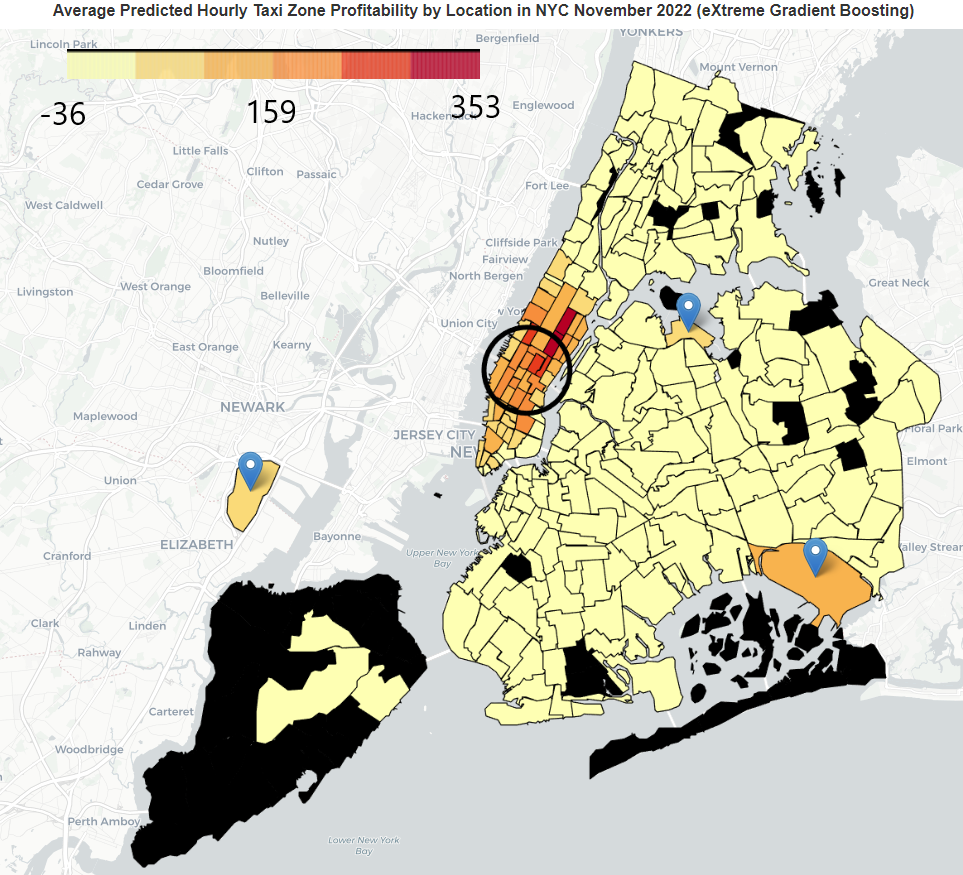
\includegraphics[width=1\linewidth]{plots/modelling_map_XGB_edit.png}  
    \caption{XGBoost}
    \label{3c}
\end{subfigure}
\caption{Actual vs Predicted Hourly Zone Profitability November 2022}
\label{3}
\end{figure}

\pagebreak

\section{Recommendations}
Based on the analysis and modelling conducted within this paper, the following recommendations are provided to taxi companies and taxi drivers:
\begin{itemize} 
    \item Taxi companies should try to incorporate the XGBoost regression model into a smart routing / dispatch system that uses the predicted hourly zone profitability to decide where taxis should be going during any given hour. Taxi companies could look to improve upon the XGBoost regression model produced by using a larger training set that covers several years and potentially even adding their own features. (Table \ref{1}) and (Figure \ref{3}) show that this model is more than suitable for the purposes of predicting zone profitability to an accurate enough level to guide taxi routing, especially in the hotspots such as the CBD and airports.
    \item Taxi drivers and taxi companies should maximise their presence in the CBD and should also avoid time spent outside of Manhattan unless they are at JFK or LaGuardia Airport based on (Figure \ref{1a}). Furthermore, it is crucial that taxi drivers spend as much time as possible near the CBD / wealthy Manhattan areas on weekdays during the morning and during rush hour when people are going to / from work as seen in (Figure \ref{1b}) and (Figure \ref{2}). There, it is highly likely that a taxi driver can rapidly complete several trips in succession during these timeframes due to the large number of people constantly using taxis to head to work. 
\end{itemize} 

\clearpage

% BEGIN REFERENCES SECTION
\printbibliography

\end{document}